\documentclass[conference]{IEEEtran}
\usepackage[utf8]{inputenc}
\usepackage[T1]{fontenc}
\usepackage{graphicx}
\usepackage{booktabs}
\usepackage{amsmath,amssymb}
\usepackage{xcolor}
\usepackage{hyperref}

% ---- figure placeholder box ----
\newcommand{\figplaceholder}[2]{%
\fbox{\parbox[c][#1][c]{0.95\linewidth}{\centering\small\textit{#2}}}}

\begin{document}

\title{Physics-Guided Calibrated Localization\\ of Methane Sources}

\author{\IEEEauthorblockN{Edward Cha, Eric Liang, and Alex Zhang}}

\maketitle

\begin{abstract}
We present a physics-guided method for localizing methane leaks from
inexpensive sensor networks, with a statistical guarantee that the
reported region contains the source 90\% of the time. The core of the
method is a set of \emph{physics input images}: for every cell of a site
map, closed-form formulas score how strongly the sensor readings point to
a leak at that cell, how visible such a leak would be to the sensor
layout, and how well the best-fitting leak rate at that cell explains the
readings. Computed in closed form, these images are supplied to a
standard neural network as additional input channels through a small
zero-initialized head (0.2\% added parameters), trained with ordinary
labels, and calibrated with split conformal prediction. When the wind is
only measured rather than known, the images are averaged over the wind
sensor's stated error range, so the network also sees how fragile each
cell's evidence is to wind error. On a testbed whose physics is exactly
solvable, so the smallest 90\%-mass region under the exact simulator
posterior is computable, the method halves the median 90\% region of a
calibrated deep localizer from 94--98\,m to 46--48\,m across three
network families, at the 50\,m scale that U.S. EPA super-emitter
notifications use to associate a leak with a facility. At a
representative 10$^\circ$/10\% anemometer-error setting, where the
evaluated measured-wind inversion baselines produce operationally
uninformative calibrated regions, the method retains its guarantee at
\textbf{68--73\,m across the same three network families}, with about
a quarter of cases below 50\,m. All results are
verified against exact references and reported over multiple training
seeds.
\end{abstract}

\begin{IEEEkeywords}
methane monitoring, conformal prediction, sensor networks, wind
uncertainty, physics-guided machine learning
\end{IEEEkeywords}

\section{Introduction}
Methane traps roughly $80\times$ more heat than CO$_2$ over its first 20
years and fades from the atmosphere within about a decade, so stopping
large leaks quickly is one of the highest-leverage climate actions
available today. A large share of oil-and-gas methane comes from a small
number of large point sources, known as super-emitters and defined by the
U.S. EPA as events of 100\,kg\,h$^{-1}$ or more \cite{epa}. Detection has advanced
rapidly: UNEP's satellite system issued over a thousand alerts in two
years \cite{unep}. The bottleneck is what happens next: connecting an
alert to a specific place that a crew can inspect. EPA's Super-Emitter Program (implementation
extended to January 2027) asks notifications to identify any facility
within \textbf{50\,m} of the estimated leak location \cite{epa}. We therefore adopt
50\,m as an operationally motivated target: a region small enough to
trigger a focused inspection.

Continuous monitoring networks, in which a few inexpensive masts
capture the plume as the wind sweeps it across the site, are where this
localization can happen. Machine learning provides instant estimates,
and split conformal prediction \cite{conformal} adds a guarantee: a
region that provably contains the true source 90\% of the time. The gap we address is twofold.
First, the guarantee speaks only to how \emph{often} the region contains
the source, not to how \emph{small} the region is, and there was
previously no practical way to measure how much smaller a guaranteed
region could have been. Second, the classical alternative of inverting the
plume physics directly requires the wind to be known exactly, while every
real site has only a wind \emph{measurement}; how each approach behaves
under that everyday mismatch had not been carefully quantified.

\textbf{Contributions.}
\begin{itemize}
\item \textbf{C1: Physics input images that carry their wind-error
budget.} For every candidate cell, closed-form formulas produce four
images: the evidence for a leak at that cell, the fragility of that
evidence across the wind sensor's stated error range, the visibility of
such a leak to the sensor layout, and the fit quality of the best leak
rate at that cell. A zero-initialized head (0.2\% added parameters)
joins the images to any base network; training is ordinary supervised
learning; split conformal prediction supplies the guarantee. At zero
error budget the images provably reduce to the classical matched-filter
pair, so one recipe covers exact and measured wind alike.
\item \textbf{C2: A measuring stick that quantifies the method's value.}
A methane testbed (CH4-T) whose physics is exactly solvable, so the
exact-model reference region is computable for every scenario and any
guaranteed localizer can be audited in meters. A verified-90\% deep
localizer delivered 94--98\,m where the reference is 6--7\,m; the
images close half of that gap on all three network families we tested
(46--48\,m).
\item \textbf{C3: Robustness under measured wind.} At the evaluated
10$^\circ$/10\% anemometer-error setting, the measured-wind inversion
baselines produce operationally uninformative calibrated regions
(essentially the whole site), while the method degrades gracefully:
each added image tightens the regions further, and all three network
families land at 68--73\,m.
\end{itemize}
Every component is standard and auditable, every number below comes
from one shared, verified simulator with identical splits and
calibration harness, and headline comparisons carry paired-bootstrap
intervals over the same 2{,}000 test scenarios.

\begin{figure}[t]
\centering
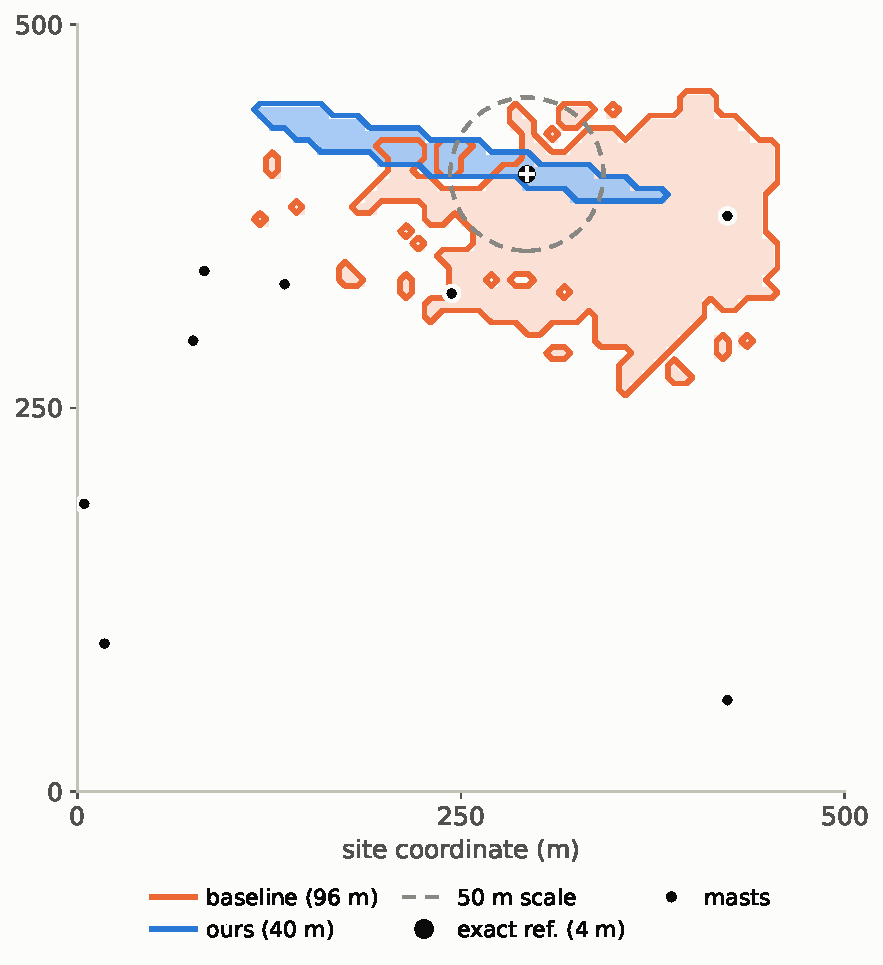
\includegraphics[width=0.4\linewidth]{../figures/paper/fig_data_example.pdf}
\caption{A well-instrumented test scenario (12 masts, measured wind):
90\% regions of the no-images baseline and of our method (conformal
masks), with the 50\,m facility scale. Selection rule: among
$\ge$10-mast scenarios whose region meets the 50\,m scale, the one at
that subset's median radius: representative of the quarter of cases
that reach the scale (Fig.~\ref{fig:dist}), not a best case.}
\label{fig:circles}
\end{figure}

\section{Related Work}
\textbf{Conformal prediction} gives distribution-free coverage
guarantees \cite{conformal}; how small the sets are is the open half of
the problem, and our audit scores it against the exact map at matched
coverage. \textbf{Simulation-based
inference} trains neural networks to approximate probability maps from
simulated data \cite{npe,sbibm}; its standard diagnostics check
calibration \cite{sbc}, and recent work examines what happens when the
simulator's settings differ from reality at deployment \cite{robsbi}. Our
measured-wind design addresses exactly that setting by building the wind
sensor's declared error range into the network's inputs. Our maps are hand-derived statistics, complementing learned summaries.
\textbf{Source-term estimation} inverts dispersion physics with
optimization or sampling at minutes to hours per event \cite{newman};
learned localizers amortize that cost into a single bounded
computation, and our audit adds the missing
instrument for judging how much information they extract.
\textbf{Controlled-release testing} (METEC) evaluates such systems in
the field \cite{metec}; our testbed mirrors that task with exact ground
truth, complementing field validation.

\begin{figure*}[t]
\centering
\figplaceholder{2.4cm}{Pipeline figure placeholder: one scenario flowing
left to right -- site sketch (masts, wind) $\rightarrow$ the four
computed physics images $\rightarrow$ set network + zero-initialized
head $\rightarrow$ the guaranteed 90\% region.}
\caption{One scenario flowing through the pipeline: sensor data
$\to$ the four computed physics images
(Eqs.~\ref{eq:zmap}--\ref{eq:resid}) $\to$ any set network with the
zero-initialized head (Eq.~\ref{eq:model}) $\to$ the guaranteed 90\%
region (Eq.~\ref{eq:region}), calibrated under the deployment wind. At
$\varepsilon{=}0$ the images reduce to the classical pair
(Eq.~\ref{eq:reduction}).}
\label{fig:pipeline}
\end{figure*}

\section{Methodology}
Our methodology has two parts. A \emph{physics simulator} makes the
truth knowable, so that every claim in this paper can be measured
rather than assumed, and records only the measured wind, so that the
evaluation matches deployment. The \emph{physics models and the
input-image method} then turn that setting into guaranteed regions:
base networks supply calibration and generalization, closed-form
physics images supply the evidence they cannot efficiently rediscover,
and split conformal prediction certifies the result.

\subsection{The physics simulator (C2)}
\label{sec:forward}
\textbf{CH4-T} places one source of unknown grid cell
$c^\ast \in \{1,\dots,64^2\}$ and rate $q$
(10--500\,kg\,h$^{-1}$, log-uniform, spanning the 100\,kg\,h$^{-1}$
super-emitter threshold) on a $500{\times}500$\,m site watched by
$S \in \{4,\dots,12\}$ masts over $T{=}30$ one-minute steps. Transport
follows the standard Gaussian plume with published
Pasquill--Gifford/Briggs dispersion (verified against the original
tables; mass conservation checked to $4{\times}10^{-6}$). In plume-frame
coordinates (downwind distance $x$, crosswind offset $y_{\mathrm{cw}}$,
sensor height $z_r$, release height $H$), the concentration per unit rate
is
\begin{equation}
\label{eq:plume}
g \;=\; \frac{1}{2\pi U \sigma_y(x)\,\sigma_z(x)}\,
e^{-\frac{y_{\mathrm{cw}}^2}{2\sigma_y^2}}
\!\left(e^{-\frac{(z_r-H)^2}{2\sigma_z^2}}
      + e^{-\frac{(z_r+H)^2}{2\sigma_z^2}}\right),
\end{equation}
where $U$ is wind speed and $\sigma_y,\sigma_z$ are the
stability-dependent dispersion widths. Stacking all sensors and time
steps, a leak at cell $c$ produces the fingerprint
$g_c(w) \in \mathbb{R}^{ST}$ under wind sequence $w$, and readings are
\begin{equation}
\label{eq:readings}
y \;=\; q\, g_{c^\ast}(w) \;+\; \epsilon, \qquad
\epsilon \sim \mathcal{N}(0,\sigma^2 I).
\end{equation}
\textbf{Wind uncertainty is built into the data.} Readings are generated
under the true wind $w$, but the dataset records only the measurement
$\hat w$, corrupted independently at every step $t$:
\begin{equation}
\label{eq:winderr}
\hat\theta_t = \theta_t + \delta_t,\quad
\hat s_t = s_t\, e^{\eta_t},\quad
\delta_t \!\sim\! \mathcal{N}(0,\sigma_\theta^2),\;
\eta_t \!\sim\! \mathcal{N}(0,\sigma_s^2),
\end{equation}
with $\sigma_\theta = 10^\circ$ and $\sigma_s = 0.10$, the accuracy class
of inexpensive monitoring anemometers. No model, at any stage, observes
the true wind.

The simulator is deliberately built so that the truth is computable.
Because the model \eqref{eq:readings} is linear in $q$, the per-cell
likelihood depends on the data only through three summary quantities,
\begin{equation}
\label{eq:suffstats}
a_c = g_c^\top y, \qquad b_c = \lVert g_c\rVert^2, \qquad
\rho = \lVert y\rVert^2,
\end{equation}
and the exact probability map under known wind follows by integrating the
rate out of the Gaussian likelihood:
\begin{equation}
\label{eq:posterior}
p(c \mid y) \;\propto\;
\int_0^{\infty}\!
\exp\!\Big(\!-\tfrac{\rho - 2qa_c + q^2 b_c}{2\sigma^2}\Big)\,
\pi(q)\, dq,
\end{equation}
evaluated by high-precision quadrature (normalization checked to
$\sim$$10^{-12}$). \textbf{The exact-model reference region.} For each
scenario we normalize \eqref{eq:posterior} over cells, using a uniform
source-cell prior and the same log-uniform rate prior $\pi(q)$ on
$[10, 500]$\,kg\,h$^{-1}$ used to generate the data (peak-aware
composite Gauss--Legendre quadrature over that range), and apply the
identical conformal wrapper of \S\ref{sec:conf} to the exact map
itself, with the same randomized tie handling and strict threshold
rule: the region is the smallest set of highest-posterior cells at the
calibrated mass threshold. We call this the \emph{exact-model reference
region}. It is an oracle reference under the CH4-T simulator
assumptions, not a universal information-theoretic lower bound. The two
reported values correspond to different coverage levels: 7.0\,m at
nominal 90\% (empirical 0.952; the exact map is conservative on the
discrete grid) and 6.2\,m at the learned models' matched empirical
coverage of 0.89. A blocking check requires the wrapper applied to the
exact map to reproduce its own guarantee before any experiment
proceeds; this check caught two real implementation bugs, including a
tie-handling correction that we report for reuse.

\subsection{The physics models and the input-image method (C1)}
\label{sec:models}

\textbf{Base learners.}
A monitoring system must answer within its observation window, on
whatever layout a site has, under the wind it actually measured. A
network trained once on simulated scenarios answers at negligible,
bounded cost per scenario and,
because it learns from examples, absorbs regularities with no closed
form, such as how anemometer error distorts the evidence. The readings form a \emph{set} of tokens (mast
position, time, concentration, wind step) whose size varies from site to
site, so the natural base learners are permutation-invariant set
networks. We evaluate three families with different inductive biases,
DeepSets (pooling), a graph neural network (relational structure between
masts), and a Set Transformer (attention), precisely so that the
method's value is demonstrated independently of any one architecture
choice.

\textbf{The physics input images.}\label{sec:maps} The plume model \eqref{eq:plume}--\eqref{eq:readings} fixes an exact
relationship between any hypothesized leak and the readings it should
produce, so testing a hypothesis is a correlation computation. The
controlled comparisons of \S\ref{sec:est} show that networks trained
end-to-end do not efficiently reconstruct this computation across
4{,}096 candidate cells (a correctly calibrated baseline delivers
94--98\,m), while the computation by itself cannot judge how much to
trust its own answer (calibrated alone, it returns the whole site). We
therefore insert an \emph{input processor} between the raw data and the
network (Fig.~\ref{fig:pipeline}): it evaluates the physics
relationships explicitly, cell by cell, and presents the results as
images aligned with the output grid,
where a small convolutional head can read them spatially. This is the
division of labor the paper centers on: physics supplies exact
understanding of how a leak maps to readings, and the network supplies
what physics lacks, calibration and generalization learned from
examples. The classical matched-filter score of cell $c$ normalizes the
alignment $a_c$ by the fingerprint's energy,
\begin{equation}
\label{eq:zmap}
z_c \;=\; \frac{a_c}{\sigma \sqrt{b_c}},
\end{equation}
and $\log b_c$ records how visible a leak at $c$ would be to the current
sensor layout. These two $64{\times}64$ images are the zero-budget input
maps. To carry the wind sensor's stated error range, we draw $K{=}8$
plausible true winds from the error model \eqref{eq:winderr} centered on
the measurement,
\begin{equation}
\label{eq:draws}
w^{(k)} \sim \mathcal{E}_{\varepsilon}(\hat w), \qquad k = 1,\dots,K,
\end{equation}
recompute \eqref{eq:suffstats} under each draw, and feed four images: the
average evidence and its variability,
\begin{equation}
\label{eq:moments}
\bar z_c = \frac{1}{K}\sum_{k} z_c^{(k)}, \qquad
v_c = \Big(\tfrac{1}{K}\sum_{k}\big(z_c^{(k)} - \bar z_c\big)^2\Big)^{1/2},
\end{equation}
the average sensitivity $\overline{\log b_c}$, and the average
\emph{fit quality}. For each draw, the best nonnegative rate at cell $c$
is $\hat q_c = \max(0, a_c/b_c)$, and the residual error it leaves is
available in closed form,
\begin{equation}
\label{eq:resid}
R_c^{(k)} \;=\; \rho \;-\; 2\hat q_c a_c^{(k)} \;+\; \hat q_c^2 b_c^{(k)},
\qquad
\bar R_c = \frac{1}{K}\sum_k R_c^{(k)},
\end{equation}
normalized per scenario (shifted to minimum zero, scaled by the median,
clipped) so that all leak rates share one scale. Every image is
closed-form linear algebra computed from the network's own inputs.
The full pipeline is a bounded, non-iterative computation whose cost
is countable from the formulas: the images require
$K \cdot |\mathcal{C}| \cdot S \cdot T$ closed-form plume evaluations
plus small inner products, on the order of $10^8$ floating-point
operations per scenario at the tested configuration, and inference is
one forward pass of a 4.9M-parameter network. One scenario consumes a
30-minute observation window, so this workload sits orders of magnitude
below the per-second throughput of any commodity processor: deployment
requires neither a GPU nor per-event optimization, in contrast to
sampling-based inversion at minutes to hours per event \cite{newman}. We verified \eqref{eq:resid} against direct
reconstruction to relative error $10^{-7}$.

\textbf{Zero-budget reduction.} With $\varepsilon = 0$ there is a single
wind, so $v_c \equiv 0$, and the fit-quality image collapses onto the
evidence image through the identity
\begin{equation}
\label{eq:reduction}
R_c \;=\; \rho \;-\; \sigma^2 \max(z_c, 0)^2,
\end{equation}
a fixed per-scenario transformation of $z_c$. The four images therefore
carry exactly the information of the classical pair $(z_c, \log b_c)$:
one recipe covers both settings, and the exact-wind results below are its
zero-budget instantiation.

\textbf{Training and the guarantee.}\label{sec:conf} The input
processor attaches to any base learner $f_\theta$ over the
token set $x$ through a three-layer convolutional head $h_\phi$
($\sim$10k parameters, 0.2\% of the model) that reads the map stack
$M(x)$, joined at the output logits:
\begin{equation}
\label{eq:model}
\ell(x) \;=\; f_\theta(x) \;+\; h_\phi\big(M(x)\big), \qquad
\hat p(c \mid x) = \mathrm{softmax}\big(\ell(x)\big)_c,
\end{equation}
with $h_\phi$ initialized at exactly zero, so at the first training step
the model is the unmodified baseline and every comparison is controlled
by construction. Training is ordinary supervised learning on smoothed
one-hot targets $t(x)$:
\begin{equation}
\label{eq:loss}
\mathcal{L}(\theta,\phi) \;=\;
-\sum_{c} t_c(x)\, \log \hat p(c \mid x).
\end{equation}
Physics enters only through the inputs in \eqref{eq:model}.

For the guarantee we use split conformal prediction with a randomized
highest-probability score. For a scenario with true cell $c^\ast$, the
score is the probability mass ranked strictly above the true cell, plus a
uniform share $u \sim \mathrm{Unif}[0,1]$ of the tied mass:
\begin{equation}
\label{eq:score}
s(x, c^\ast) \;=\;
\sum_{c:\, \hat p_c > \hat p_{c^\ast}} \hat p_c
\;+\; u \sum_{c:\, \hat p_c = \hat p_{c^\ast}} \hat p_c .
\end{equation}
The threshold $\hat t$ is the $\lceil (n{+}1)(1{-}\alpha)\rceil$-th
smallest score over $n$ calibration scenarios ($\alpha = 0.1$), and the
region keeps the most probable cells, excluding only mass strictly below
the threshold (the tie-handling correction of \S\ref{sec:forward}):
\begin{equation}
\label{eq:region}
\mathcal{R}(x) = \big\{c : s(x,c) \le \hat t\,\big\},
\qquad
\Pr\big[c^\ast \in \mathcal{R}(x)\big] \;\ge\; 1 - \alpha .
\end{equation}
Calibration is always performed under the same wind condition in which
the system is evaluated, so \eqref{eq:region} certifies the deployment
setting. Region sizes are reported as the radius of the circle of equal
area; all models share identical data (10k/1k/2k/2k splits, a standard
budget for this field \cite{sbibm}) and identical symmetry augmentation.

\textbf{Scope of the guarantee.} The conformal guarantee
\eqref{eq:region} is marginal over exchangeable scenarios drawn from the
calibration distribution; it does not imply 90\% coverage for every
individual scenario, leak-rate range, sensor layout, or wind
condition. Calibration is performed separately for each evaluated
deployment condition. The exact-model reference only audits efficiency under the testbed
assumptions and is not part of the guarantee.

\textbf{Division of labor.} The physics computes exact per-cell
evidence through \eqref{eq:zmap}--\eqref{eq:resid}, knowledge a network
would otherwise have to rediscover from data; the network, trained
through \eqref{eq:loss}, generalizes across layouts, rates, and wind
histories and learns how much to trust each cell's evidence, knowledge
with no closed form; conformal calibration \eqref{eq:region} certifies
the result.

\textbf{The pipeline, end to end.} For each scenario:
(1)~from the measured wind and its stated error budget, draw $K$
plausible winds and compute the four images
\eqref{eq:zmap}--\eqref{eq:resid}, closed-form summaries of what the
physics says about every candidate cell; (2)~feed the images, alongside
the raw sensor tokens, to the base network through the zero-initialized
head \eqref{eq:model}, so training starts from the unmodified baseline
and the network learns from labels alone how much to trust each cell's
physics evidence given the layout, leak rate, and wind at hand;
(3)~calibrate with split conformal under the deployment condition
\eqref{eq:region}. Performance improves for a simple reason: the
network no longer has to rediscover the evidence computation from
finite data: it starts from exact per-cell physics and spends its
capacity on the corrections that have no closed form, which is why the
gains grow as the images carry more of the wind-error structure.


\section{Results}
\subsection{The audit, in the laboratory limit}
\label{sec:est}
Both learned pipelines pass every standard calibration check (coverage
0.89 at nominal 90\%); only the audit reveals what calibration alone
cannot. The labels-only baseline delivers 94--98\,m where the
exact-model reference is 6.2--7.0\,m, more than ten times the
reference; two input images and a small head close half of the
distance, to 47.1--47.7\,m. Relative to the labels-only
model on the same 2{,}000 paired scenarios, the images reduce the median
radius by 46.1\,m (paired-bootstrap 95\% CI $[43.6, 48.1]$), produce
smaller regions in 96.4\% of cases, and place 52.4\% of regions below
the 50\,m scale (Clopper--Pearson 95\% CI $[50.2, 54.6]$\%).

The fix is architecture-independent (Table~\ref{tab:est}): three
network families with a 40\,m baseline spread land inside a 1.5\,m
band once the images are supplied, so the gain is available to whatever
architecture a practitioner already has.

\begin{table}[t]
\centering
\caption{The physics images help every model (median 90\% region
radius in m; laboratory limit; 3 seeds per cell; coverage 0.88--0.92
throughout).}
\label{tab:est}
\begin{tabular}{lcc}
\toprule
Base network & Without images & With images \\
\midrule
DeepSets        & 94--98 & \textbf{47.1--47.7} \\
GNN             & 56--57 & \textbf{46.2--47.5} \\
Set Transformer & 69--71 & \textbf{46.2--47.3} \\
\bottomrule
\end{tabular}
\end{table} The classical score alone, calibrated with no network, is
overconfident-wrong and returns essentially the full site. All
remaining results are reported under the simulator's native condition:
measured wind.

\subsection{Measured wind: the main results}
\label{sec:robust}
\begin{table}[t]
\centering
\caption{The physics images help every model under measured wind
($10^\circ$/10\% per-step anemometer error; 3 seeds per cell; coverage
0.89--0.92 with images. For reference, direct physics inversion retains
its guarantee only at coverage 1.00, returning the full site, 282\,m.)}
\label{tab:wind}
\setlength{\tabcolsep}{3.5pt}
\footnotesize
\begin{tabular}{lcccc}
\toprule
 & \multicolumn{2}{c}{Without images} &
\multicolumn{2}{c}{With images} \\
Base network & Radius (m) & $<$50\,m & Radius (m) & $<$50\,m \\
\midrule
DeepSets & 107.9--110.5 & 0\% & \textbf{70.1--72.9} & 24--27\% \\
GNN & 69.2--71.3 & 1--5\% & \textbf{68.4--69.3} & 27--29\% \\
Set Transformer & 80.4--82.3 & 7--12\% & \textbf{69.4--70.3} & 26\% \\
\bottomrule
\end{tabular}
\end{table}

\begin{table}[t]
\centering
\caption{Cumulative image ablation under measured wind (DeepSets base;
3 seeds per row). Each of the four images is added on top of the
previous ones; the fragility step also draw-averages the first two
images (Eq.~\ref{eq:moments}).}
\label{tab:comp}
\setlength{\tabcolsep}{4pt}
\begin{tabular}{lccc}
\toprule
Input images & Cov. & Radius (m) & $<$50\,m \\
\midrule
none (input-only network) & 0.90--0.91 & 107.9--110.5 & 0\% \\
+ evidence image ($\bar z_c$) & 0.90 & 87.7--88.5 & 12\% \\
+ sensitivity image ($\overline{\log b_c}$) & 0.91--0.92 & 82.2--84.2
& 15--17\% \\
+ wind-fragility image ($v_c$) & 0.89--0.91 & 74.7--76.3 & 20--21\% \\
\textbf{+ fit-quality image ($\bar R_c$)} & 0.90--0.92 &
\textbf{70.1--72.9} & \textbf{24--27\%} \\
\bottomrule
\end{tabular}
\end{table}

\begin{figure}[t]
\centering
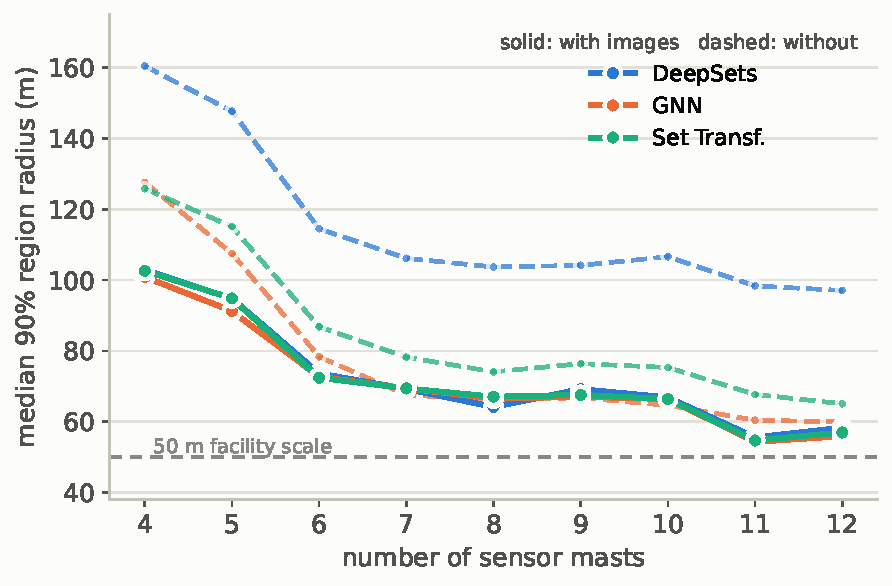
\includegraphics[width=0.7\linewidth]{../figures/paper/fig_data_masts.pdf}
\caption{Sensor-count ablation (measured wind, seed-1 diagnostic;
$\approx$210--240 test scenarios per mast count). More masts shrink the
guaranteed regions toward the facility scale; the conformal guarantee
remains marginal over the full distribution.}
\label{tab:masts}
\end{figure}

\begin{figure}[t]
\centering
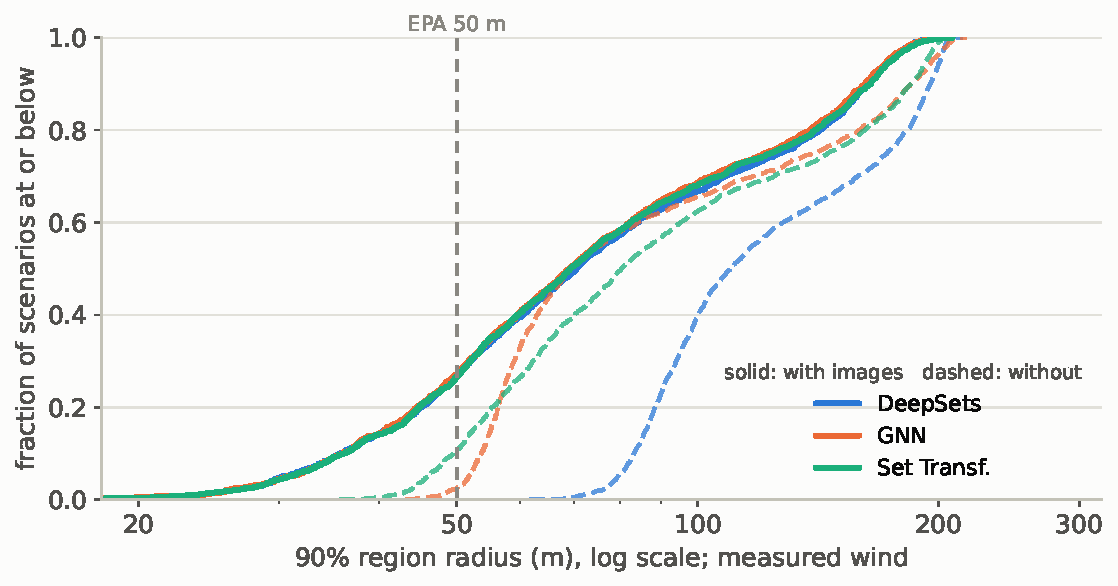
\includegraphics[width=0.68\linewidth]{../figures/paper/fig_data_dist.pdf}
\caption{Region-radius distributions over all 2{,}000 test scenarios
under measured wind: 27\% of our regions fall below the 50\,m scale
while the median sits at 71\,m; the no-images distribution never
reaches the scale.}
\label{fig:dist}
\end{figure}

Real anemometers have error, and the effect on direct physics inversion
is dramatic. Trusting the measured wind exactly, it concentrates its
probability so far from the true source that, to keep its guarantee, the
calibration wrapper must return essentially the entire site
(282\,m at coverage 1.00); allowing extra measurement noise, tuned on
held-out data, does not change this. A negative control isolates the
cause of our gains: feeding the identical head four \emph{random} images
of the same shape and scale (one seed, diagnostic) matches
the no-physics baseline (107.5\,m), so the improvement traces to the
physics content of the images, not to added capacity or spatial
regularization. The learned recipe behaves differently, and the pattern
is clean: the more of the wind sensor's
error-range information the input images carry, the smaller the
guaranteed regions become (Table~\ref{tab:comp}): from 82--84\,m using
the measured wind alone, to 74--76\,m after adding the moment images
\eqref{eq:moments}, to \textbf{70--73\,m} after adding the fit-quality
image \eqref{eq:resid}.
Relative to the no-physics model on the same 2{,}000 paired scenarios,
the full method reduces the median radius by 39.4\,m (paired-bootstrap
95\% CI $[37.3, 41.9]$), produces smaller regions in 96.2\% of cases,
and places 26.6\% of regions below 50\,m (Clopper--Pearson 95\% CI
$[24.7, 28.6]$\%). Throughout, this is one network, one objective \eqref{eq:loss}, one
guarantee \eqref{eq:region}, one forward pass. The mechanism is constructive: because the physics and the
sensor's own error range live in the inputs, ordinary supervised
training gives the network thousands of examples from which to learn how
the error behaves and how much to trust each cell's evidence. In summary: $94{\to}47$\,m from supplying a missing
computation; $47{\to}71$\,m, the measured cost of imperfect wind;
$108{\to}71$\,m, the value of physics in the inputs at this setting.

\section{Limitations}
CH4-T is a measuring instrument, not a deployment: single steady
sources, flat terrain, known stability class, and a 64$\times$64 grid
whose $\sim$7.8\,m cells sit near the reference scale. The 6--7\,m
reference is a property of the testbed's assumptions, exists only under
known wind (the measured-wind analogue is not computable, so 70--73\,m
is reported against the 50\,m operational scale), and the wind error
range is taken as known from the instrument specification; quantifying
sensitivity to a misspecified range is a natural next step. In the laboratory limit, roughly half of individual cases still
exceed
50\,m (p90\,$=$\,131\,m); prespecified subgroup diagnostics show no
collapsing group, with mild under-coverage for sparse-mast scenarios as
the one consistent pattern (coverage 0.865--0.867 at 4--6 masts,
$n{=}690$, about 3 standard errors below nominal), a concrete target for
group-conditional calibration. Field validation on
controlled releases is the natural next stage, and the comparisons
reported here are exact regardless, because every method shares one
verified simulator, one dataset, and one calibration harness.

\section{Conclusions}
On a testbed with exact ground truth, a calibrated deep localizer
delivered a tenth of the sharpness of the exact-model reference.
Supplying one classical computation as input images brought three
network families to 46--48\,m at the 50\,m facility-association scale,
and the same recipe, carrying the wind sensor's stated error range in
its inputs, retained its guarantee at 70--73\,m at the evaluated
anemometer-error setting, at a bounded, non-iterative computational
cost with 0.2\% added parameters.

The research impact is a transferable evidence standard: exactly
solvable testbeds as measuring instruments for learned inference,
self-checking calibration gates, and one-change-at-a-time controls,
applicable wherever guaranteed regions are produced. The social impact
is practical: regions small enough to act on, produced well within
each observation window on commodity hardware, with stated guarantees and the wind sensor's
imperfection budgeted honestly. This provides a controlled step toward
converting methane detections into calibrated inspection regions.

{\footnotesize
\begin{thebibliography}{12}
\bibitem{unep} UN Environment Programme (IMEO), ``An Eye on
Methane,'' 2024.
\bibitem{epa} U.S. EPA, ``Standards of performance for GHG emissions:
NSPS OOOOb/EG OOOOc and the Super-Emitter Program,'' 89 FR 16820, 2024;
implementation timing per the 2025 Interim Final Rule.
\bibitem{conformal} A.~N. Angelopoulos and S.~Bates, ``Conformal
prediction: A gentle introduction,'' \emph{Found. Trends Mach. Learn.},
16(4), 2023.
\bibitem{sbc} S.~Talts \emph{et al.}, ``Validating Bayesian inference
algorithms with simulation-based calibration,'' arXiv:1804.06788, 2018.
\bibitem{npe} G.~Papamakarios and I.~Murray, ``Fast $\varepsilon$-free
inference of simulation models with Bayesian conditional density
estimation,'' \emph{NeurIPS}, 2016.
\bibitem{sbibm} J.-M. Lueckmann \emph{et al.}, ``Benchmarking
simulation-based inference,'' \emph{AISTATS}, 2021.
\bibitem{robsbi} P.~Cannon, D.~Ward, and S.~M. Schmon, ``Model
misspecification in neural simulation-based inference,''
arXiv:2209.01845, 2022.
\bibitem{newman} T.~Newman \emph{et al.}, ``Probabilistic inversion
modeling of gas emissions,'' arXiv:2408.01298, 2024.
\bibitem{metec} C.~Ilonze \emph{et al.}, ``Assessing continuous
monitoring solutions under single-blind controlled testing,''
\emph{Elementa}, 2025.
\end{thebibliography}}

\onecolumn
\appendix
\section*{Appendix A: Full Results}
All numbers are median 90\% conformal region radii in meters over the
2{,}000-scenario test set, with empirical coverage and the fraction of
regions below the 50\,m facility scale; ranges are over 3 training seeds
unless marked $^{1s}$ (single-seed diagnostic) or $^{2s}$.

\begin{table}[h]
\centering
\caption{Exact wind ($\varepsilon=0$): all evaluated configurations.}
\begin{tabular}{llccc}
\toprule
Configuration & Estimator & Coverage & Radius (m) & $<$50\,m \\
\midrule
Exact-model reference & --- & 0.89--0.95 & 6.2--7.0 & 72\% \\
Labels only & DeepSets & 0.890 & 94--98 & 0\% \\
Labels only & GNN & 0.881--0.904 & 56.3--57.4 & 36--39\% \\
Labels only & Set Transformer & 0.888--0.894 & 68.7--70.8 & 18--22\% \\
+ physics images & DeepSets & 0.888--0.895 & 47.1--47.7 & 52--53\% \\
+ physics images & GNN & 0.891--0.902 & 46.2--47.5 & 53--54\% \\
+ physics images & Set Transformer & 0.892--0.901 & 46.2--47.3 & 53--54\% \\
Flow-based estimator & spline flow & 0.90--0.91 & 62.8--71.2 & 19--37\% \\
Flow + physics images & spline flow & 0.89--0.91 & 57.6--61.2 & 37--42\% \\
Classical score alone & no network & 1.00 & 282 (full site) & 0\% \\
\midrule
Channel ablation: evidence only & DeepSets & 0.88 & 65.0$^{1s}$ & 33\% \\
Channel ablation: sensitivity only & DeepSets & 0.90 & 98.5$^{1s}$ & 0\% \\
\bottomrule
\end{tabular}
\end{table}

\begin{table}[h]
\centering
\caption{Measured wind ($10^\circ$/10\% per-step anemometer error; no
method observes the true wind; calibration under the deployment
condition).}
\begin{tabular}{lccc}
\toprule
Configuration & Coverage & Radius (m) & $<$50\,m \\
\midrule
Direct physics inversion & 1.00 & 282 (full site) & 0\% \\
Inversion, tuned noise inflation ($c^\ast{=}1.5$) & 1.00 & 282 (full site) & 0\% \\
Network, no physics images & 0.898--0.907 & 107.9--110.5 & 0\% \\
Random images, identical head$^{1s}$ & 0.889 & 107.5 & 0\% \\
Ours, single-wind images & 0.911--0.920 & 82.2--84.2 & 15--17\% \\
Ours, + moment images & 0.894--0.906 & 74.7--76.3 & 20--21\% \\
Ours, full (+ fit quality) & 0.900--0.919 & 70.1--72.9 & 24--27\% \\
\midrule
Training-condition ablation: & & & \\
~~single-wind images, trained exact wind & 0.908--0.912 & 84.1--85.1 & 21--22\% \\
~~single-wind images, trained both conditions$^{2s}$ & 0.907--0.917 & 83.2--84.0 & 18\% \\
\bottomrule
\end{tabular}
\end{table}

\begin{table}[h]
\centering
\caption{Rate-stratified performance of the recipe (exact wind, seed 1).}
\begin{tabular}{lrrr}
\toprule
Leak rate (kg\,h$^{-1}$) & $n$ & Median radius (m) & $<$50\,m \\
\midrule
10--30 & 582 & 44.8 & 54\% \\
30--100 & 585 & 44.5 & 55\% \\
100--250 & 483 & 50.3 & 49\% \\
250--500 & 350 & 55.2 & 41\% \\
\bottomrule
\end{tabular}
\end{table}

\begin{table}[h]
\centering
\caption{Subgroup diagnostics (prespecified groups; seed-1 runs). These are diagnostic; the formal conformal guarantee remains marginal over the complete test distribution.}
\label{tab:subgroup}
\begin{tabular}{lrrrrr}
\toprule
 & & \multicolumn{2}{c}{Exact (ours)} &
\multicolumn{2}{c}{Measured (full)} \\
Subgroup & $n$ & Cov. & Med. & Cov. & Med. \\
\midrule
4--6 masts & 690 & 0.865 & 61.2 & 0.867 & 91.2 \\
10--12 masts & 675 & 0.899 & 42.7 & 0.926 & 59.5 \\
10--100\,kg/h & 1167 & 0.881 & 43.2 & 0.913 & 80.6 \\
100--500\,kg/h & 833 & 0.904 & 53.8 & 0.881 & 61.6 \\
wind $<$ 2.5\,m/s & 1000 & 0.885 & 49.6 & 0.884 & 63.0 \\
wind $\ge$ 2.5\,m/s & 1000 & 0.896 & 46.8 & 0.916 & 79.8 \\
\bottomrule
\end{tabular}
\end{table}

\begin{table}[h]
\centering
\caption{Reproducibility summary; full configuration and code in the project repository.}
\begin{tabular}{llll}
\toprule
Setting & Value & Setting & Value \\
\midrule
Split & 10k/1k/2k/2k & Optimizer & AdamW, lr $3{\times}10^{-4}\!\to\!3{\times}10^{-5}$ cosine, wd $10^{-4}$ \\
Site, grid & 500\,m; $64^2$ (7.8\,m cells) & Batch, epochs & 256; 200, best validation-NLL state \\
Masts & 4--12, count/positions uniform & Precision & bfloat16 autocast, grad clip 1.0 \\
Readings & 30 $\times$ 1-min averages; dropout $\le$20\% & Targets & one-hot, Gaussian-smoothed $\sigma{=}0.75$ cells; D4 \\
Noise $\sigma$ & log-uniform 0.2--3\,ppm, iid & $z$, $\log b$ normalization & clip $\pm$60, $\div$10; $(\log_{10}b{+}8)/6$ \\
Leak rate & log-uniform 10--500\,kg\,h$^{-1}$ & Residual normalization & min-shift, median-scale, clip 10 \\
Wind & speed log-unif.\ 1--8\,m\,s$^{-1}$; AR(1) $\rho{=}0.7$ & Parameters & 4.88\,M total; head 10{,}721 (0.22\%) \\
Meander & 20--40$^\circ$ dir., 10--30\% speed & Seeds & fixed data root; training 1--3; fixed score seed \\
Stability & PG classes A--F, uniform & Hardware & NVIDIA L40S \\
Wind error & $10^\circ$ dir., 10\% speed, per step & Timing (measured, our hw) & GPU 30.4\,ms; CPU 0.49\,s med \\
\bottomrule
\end{tabular}
\end{table}


\textbf{Reading the ablations.} Both physics images contribute and the
evidence image (the correlation computation) carries most of the gain;
the sensitivity image alone, which never touches the readings, adds
little over the baseline. The classical score without a network is
overconfident-wrong and pays with full-site regions, so the learned
calibration is load-bearing. The random-image control matches the
no-physics baseline, so the improvement traces to the physics content of
the images rather than to added parameters or spatial regularization.
The training-condition ablation shows the measured-wind gains come
mainly from the images themselves rather than from training under the
deployment condition.

\section*{Appendix B: Paired Bootstrap Details}
For each comparison, both methods are evaluated on the same 2{,}000 test
scenarios; we resample scenarios jointly (10{,}000 bootstrap draws), so
every draw contains paired results, and report the difference of median
radii with percentile 95\% intervals. Fractions below 50\,m carry exact
Clopper--Pearson 95\% intervals. Exact wind, labels-only vs.\ recipe:
median reduction 46.1\,m, CI $[43.6, 48.1]$; 96.4\% of scenarios
improved; 52.4\% below 50\,m, CI $[50.2, 54.6]$\%. Measured wind,
no-physics vs.\ full method: median reduction 39.4\,m, CI
$[37.3, 41.9]$; 96.2\% improved; 26.6\% below 50\,m, CI
$[24.7, 28.6]$\%.

\section*{Appendix C: Additional Result Figures}

\begin{figure}[h]
\centering
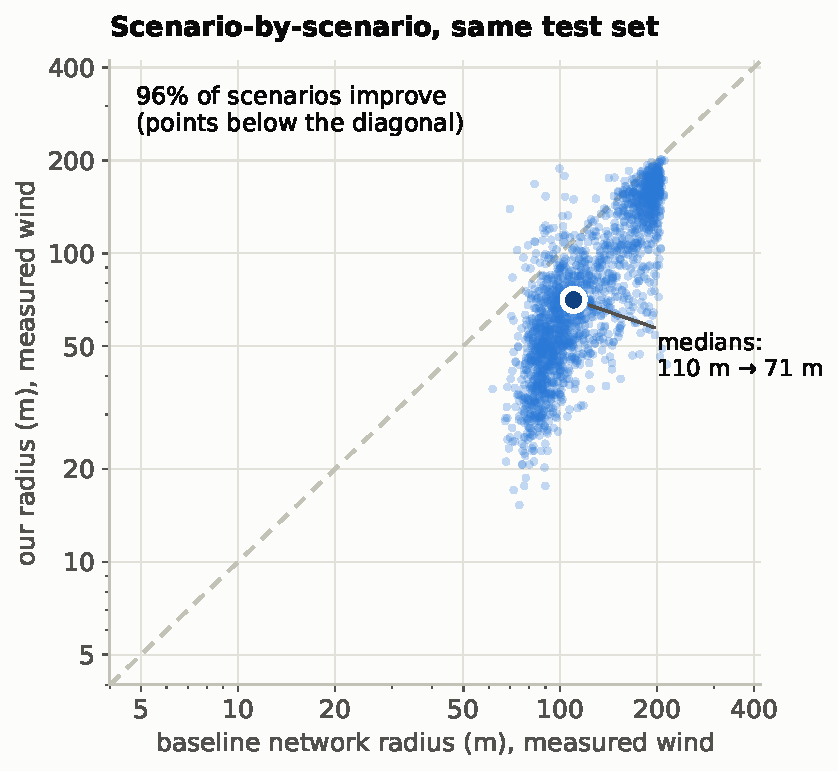
\includegraphics[width=0.5\linewidth]{../figures/paper/fig_data_scatter.pdf}
\caption{Scenario-by-scenario paired comparison under measured wind
(same 2{,}000 test scenarios): 96\% of points lie below the identity
line; medians 110\,m $\to$ 71\,m.}
\end{figure}

\begin{figure}[h]
\centering
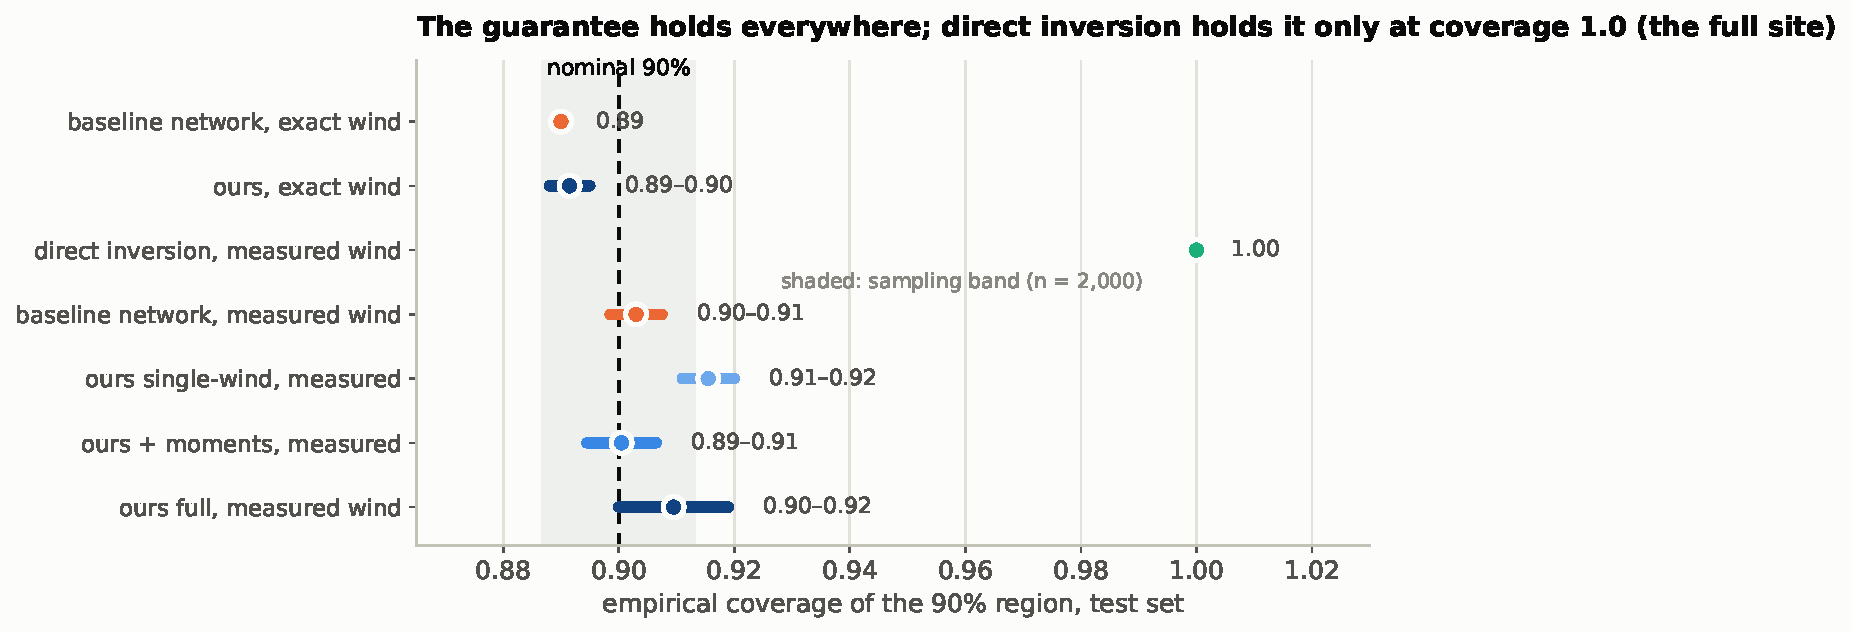
\includegraphics[width=0.72\linewidth]{../figures/paper/fig_data_coverage.pdf}
\caption{The guarantee check: empirical coverage of every configuration
against the nominal 90\% line with the $n{=}2{,}000$ sampling band.
Direct inversion holds its guarantee only at coverage 1.0, i.e., by
returning the full site.}
\end{figure}

\begin{figure}[h]
\centering
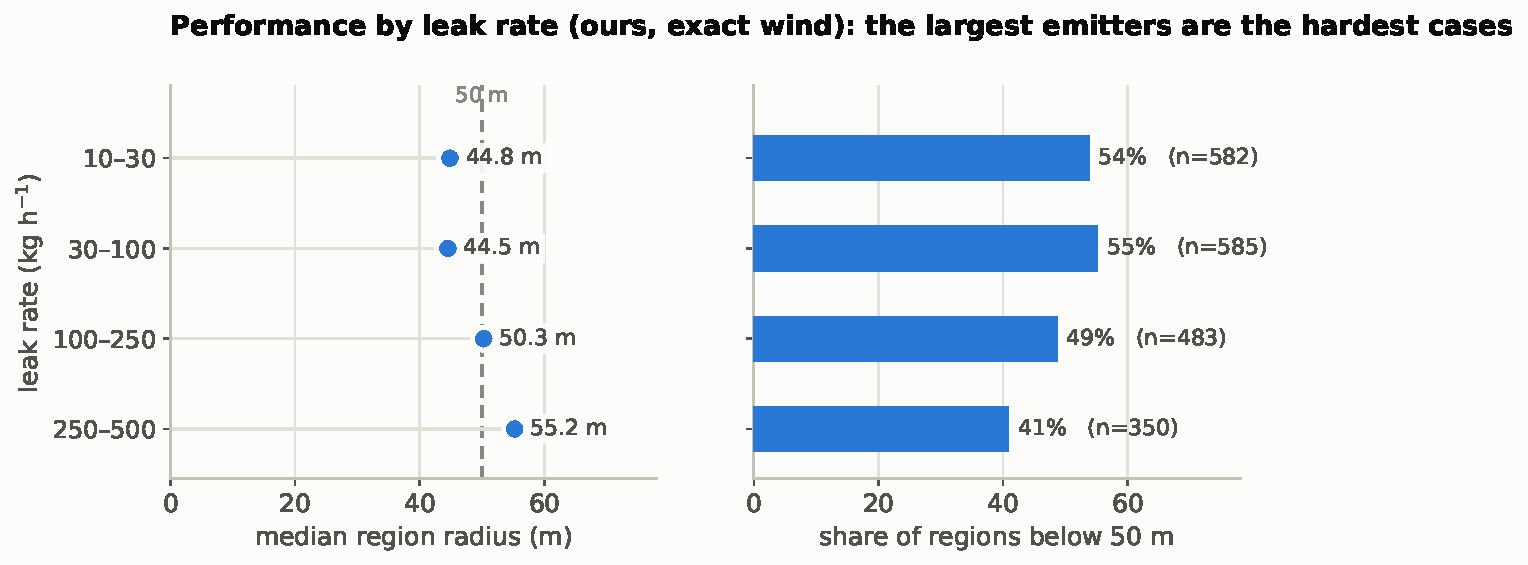
\includegraphics[width=0.72\linewidth]{../figures/paper/fig_data_rates.pdf}
\caption{Performance by leak rate (ours, exact wind): the largest
emitters are the hardest cases.}
\end{figure}

\begin{figure}[h]
\centering
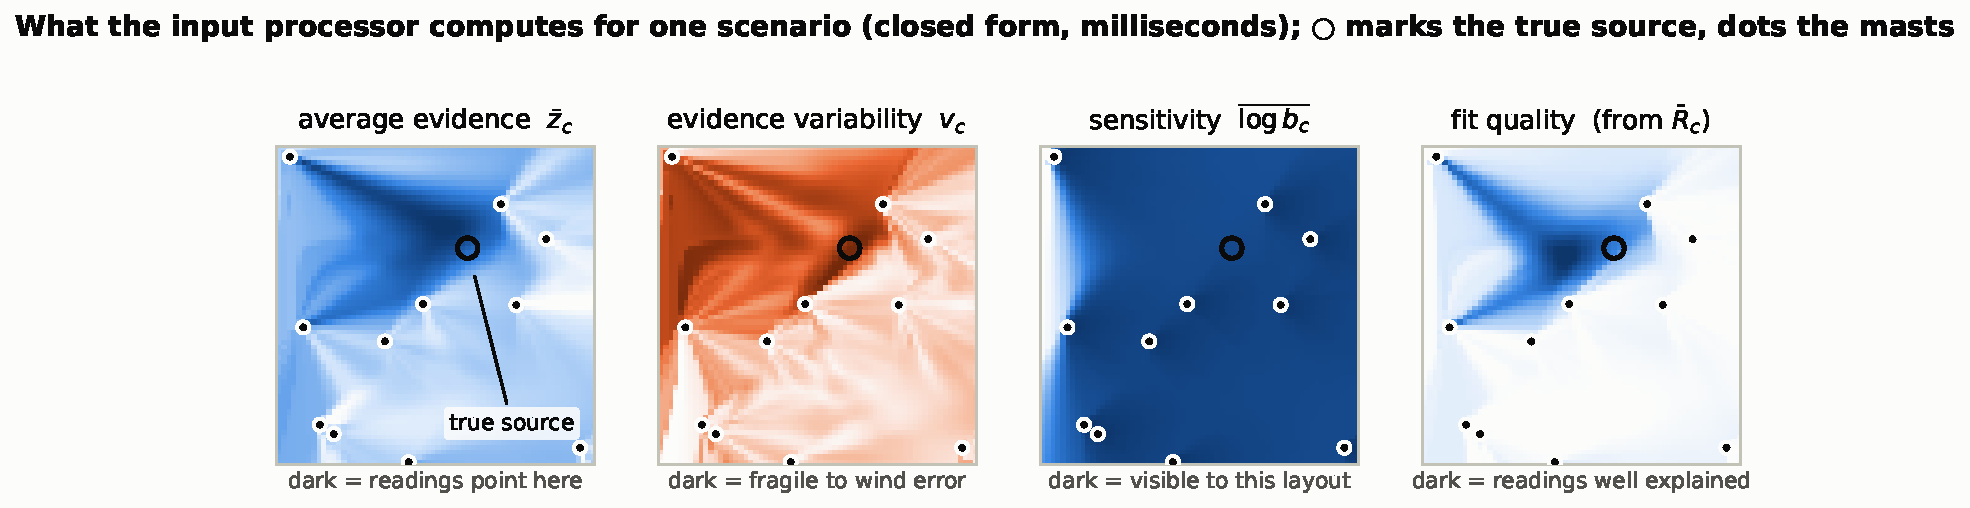
\includegraphics[width=0.95\linewidth]{../figures/poster/poster_maps.pdf}
\caption{The four physics input images for one test scenario (closed
form, computed from the network's own inputs at the measured wind):
average evidence, evidence variability across the wind-error range,
sensitivity, and fit quality. The circle marks the true source; dots
mark the sensor masts.}
\end{figure}


\end{document}
